\section{Introduction}

Explosive phenomenas that occur on the surface of sun are called as solar flares, caused by the reconnection of a sun's magnetic field lines. These flares are often accompanied by filaments/prominent eruptions and Coronal Mass Ejections (CMEs). Filaments and prominences are fundamentally of the same physical properties, only difference is the angle at which it is observed. If plasma floats outside the solar limb, it is called prominence, it is called a filament if it is within the solar background otherwise. Difference is in the type of spectrum obtained, which is Balmer lines in emission spectra in case of prominence and absorption lines in case of filaments. Loop-like structures of plasma stand out brightly against the dark background of space, these are prominences. Some prominences appear dark compared to the bright background of the Sun, these are nothing but the filaments. CME is the eruption of magnetized plasma into the Interplanetary/Interstellar Medium which were discovered in 1971. Stellar flares are also associated with CMEs, but it is not easy to detect or study them as there is no spatial resolution unlike Sun. Efforts have been done to find indirect methods of detecting and analysing stellar CMEs. Some of the methods like Coronal Dimmings, Radio Bursts, blue-shifted chromospheric lines etc. have been employed to study stellar CMEs. Time series plot of irradiance value of Sun shows a prominent decrease after the event compared to the value before the event. This effect is known as Coronal Dimming. The amount of depth and slope of the curve of the CME have been analysed to get information about the mass and velocity of the CMEs \citep{Mason2016}.

\subsection{Instrument}

\begin{figure}[ht]
    \centering
    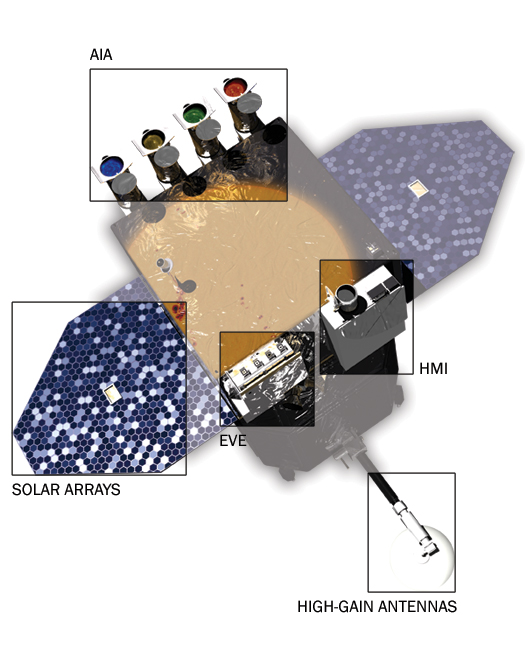
\includegraphics[width=0.5\textwidth]{images/spacecraft_detailed.jpg}
    \caption{Solar Dynamics Observatory Spacecraft.
      Image obtained from {\url{https://sdo.gsfc.nasa.gov/mission/spacecraft.php}}}
    \label{fig:label}
\end{figure}

We are using Atmosphere Imaging Assembly (AIA) instrument of Solar Dynamics Observatory (SDO) for the Sun's spectral irradiance data. SDO is a space observatory launched by NASA on 2010 as a part of `Living With a Star' (LWS) program. The spacecraft contains three instruments on board: Extreme Ultraviolet Variability Experiment (EVE), Helioseismic and Magnetic Imager (HMI), Atmospheric Imaging Assembly (AIA). We'll be focusing on the AIA instrument, since that is what we will be using. AIA was built in partnership with Lockheed Martin Solar and Astrophysics Laboratory (LMSAL). AIA contains 4 cassegrain telescopes which are optimized to observe narrow bands in the EUV region. Each of the four f/20 telescope has a 20-cm primary mirror and an active secondary mirror. The telescope is designed to prevent charged particles from reaching the Charge Coupled Device (CCD). Field of View (FOV) of each of the telescope is 41 arcmin in circular diameter. The mirrors have special multilayer coatings that are optimized to observe the selected EUV wavelengths of interest. Three of the telescopes have two different EUV bandpasses. The CCDs are back-thinned and back-illuminated with 4096 $\times$ 4096 pixels capturing capabilities. Each of the 12 $\mu$m pixel corresponds to 0.6 arcsec. The telescopes have a selector mechanism to choose the wavelength. AIA captures full-frame EUV image and one UV or visible-light image every 12 seconds. \citep{Lemen2011}

\begin{table}[h!]
    \centering
      \setlength{\tabcolsep}{10pt}
      \renewcommand{\arraystretch}{1.5}
    \begin{tabular}{| l | l | l | l |}
      \hline
       \textbf{Band} & \textbf{Primary role, ion(s)} & \textbf{Region of Sun's atmosphere} & \textbf{logT{[}K{]}} \\
      \hline
      \multirow 6173 Å & HMI scans Fe I 6173  & Intensity, velocity and & 3.7 & & & magnetic field of photosphere & \\
      \hline
      4500 Å & Continuum            & Photosphere                                            & 3.7                                   \\
      \hline
      1700 Å & Continumm            & Temperature minimum, photosphere                       & 3.7                                   \\
      \hline
      304 Å  & He II                & Chromosphere, transition region                        & 4.7                                   \\
      \hline
      1600 Å & C IV, continumm      & Transition region, upper photosphere                   & 5.0                                   \\
      \hline
      171 Å  & Fe IX                & Quiet corona, upper transition region                  & 5.8                                   \\
      \hline
      193 Å  & Fe XII, XXIV         & Corona and hot flare plasma                            & 6.1, 7.3                              \\
      \hline
      211 Å  & Fe XIV               & Active region corona                                   & 6.3                                   \\
      \hline
      335 Å  & Fe XVI               & Active region corona                                   & 6.4                                   \\
      \hline
      94 Å   & Fe XVIII             & Flaring regions                                        & 6.8                                   \\
      \hline
      131 Å  & Fe XX, XXIII         & Flaring regions                                        & 7.0, 7.2                              \\
      \hline
    \end{tabular}
    \caption{AIA wavelength channels. Table obtained from \url{https://aia.lmsal.com/public/instrument.htm}}
    \label{tab:aia_wav_channels}
\end{table}

\begin{figure}[h!]
    \centering
    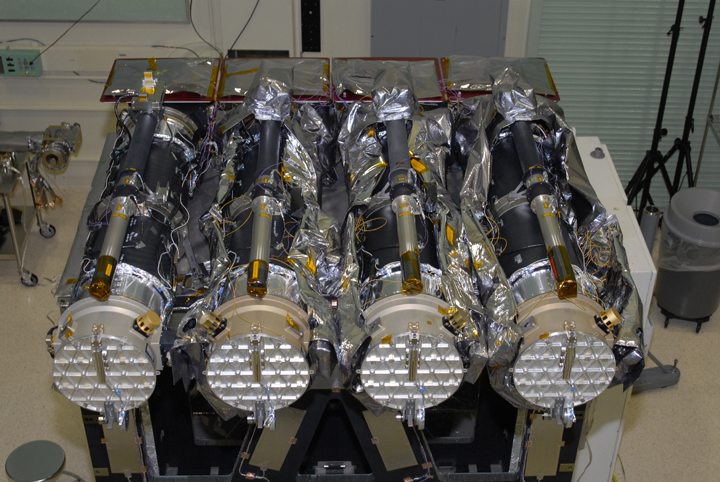
\includegraphics[width=0.5\textwidth]{images/SDO AIA Telescopes.jpg}
    \caption{SDO AIA Telescopes (Image credit: NASA)}
    \label{fig:aia_telescopes}
\end{figure}

The different channels of AIA respond differently to the radiation of different temperature. The temperature response curves gives the information about the response of each of the channels with respect to the temperature of the radiation being received. The following figure shows the response curves, which has been obtained using \texttt{aia\_get\_response.pro} procedure of SSW IDL.

\textbf{ADD TEMPERATURE RESPONSE CURVES}

%%% Local Variables:
%%% mode: LaTeX
%%% TeX-master: "main"
%%% End:
